\section{BCDI}

\subsection{Coherent diffraction}

Bragg coherent diffractive imaging (BCDI) is a lensless x-ray imaging technique that uses computational algorithms in place of physical lenses to achieve high-resolution imaging. It can be used to visualize the Bragg electron density and atomic displacement fields of crystalline materials in three-dimensional (3D) detail and with nanometer resolution.

We focus only on elastic scattering as that is the main process exploited when studying the structure of materials (the x-ray photon is elastically scattered (energy is conserved) and both the incident and scattered photons have the same wavelength).

By adding up the scattered amplitudes of an arrangement of atoms, we can then get the diffracted amplitude for a crystal. Note that the following derivations only apply if the diffraction pattern is viewed at a distance far away from the diffracting object. This region is known as the far-field or Fraunhofer region.

\subsection{Phase retrieval}

Basic algorithm is Error-Retrieval (ER), quick but can converge towards local minimum. 
The support corresponds to a shape when the object is included. The density of the object is thus equal to zero outside the support. (Fienup, 1978).

In practice, a slow convergence of the ER algorithm is often observed. The error-metric does not evolve and the algorithm is sort of stuck in a local minimum.

To overcome the problem of stagnation in local minima from ER, (FIenup, 1982) introduced the Hybrid-Input-Output algorithm, that differs in its application of real space constraints. Feedback parameter $\beta$, 
In practice, this adaptation is efficient and significantly enhances the convergence speed. It can be seen as a little perturbation that allows to leave a local minimum.


However, the HIO algorithm still fails sometimes, and this explains why the ER and HIO algorithms are generally used in combination.

\subsubsection{Support determination}
There are several techniques to estimate the support. In some cases, the shape and dimensions of the object have been already determined by other techniques (such as SEM or AFM for instance), and a support can be built from this knowledge. 

\subsubsection{Patterson function}
When the shape of the object is unknown, a rough estimate of the support can be obtained from the diffraction signal using the autocorrelation function (Marchesini 2003). It is based on the Patterson function which can be defined as the invert Fourier transform of the diffracted intensity. This function can be expressed as the convolution of the complex electron density.

The size of the crystal is overestimated by the Patterson function, since it provides its autocorrelation. In practice, a non uniform density leads to a non-trivial shape of the autocorrelation. The function needs to be threshold to start with a reasonable approximation. In most of the reconstructions in this manuscript, the threshold was set to 2\% of the maximum of the Patterson function. As discussed by Vaxelaire (2011), the method is not adapted to highly strained objects.


For large strain, the diffraction pattern has a large extent in the reciprocal space
(Beutier et al. 2013a). As a consequence, the Patterson function underestimates the size of the object, preventing any chance of success in the phase-retrieval procedure. In summary, if the shape and size of the object is unknown, it is not recommended to use the autocorrelation function as a first estimate of the support in the case of an highly strained system.

In combination of the ER and HIO algorithms, a third algorithm is routinely used for CDI. It is known as the shrink wrap (SW) algorithm and allows to update the support during the reconstruction. It was first introduced by Marchesini (2003) and has proven to greatly improve the convergence of the procedure.

In practice, the estimate is smoothed by convolution with a Gaussian. After convolution, a thresholding is applied to the smoothed image to a typical value of 10\% of the maximum value of the amplitude. Values above the threshold are set to 1 and values below are set to 0. The threshold is generally set to such low values to avoid to suppress too large parts of the support. Nevertheless, the convolution step allows to recover from a support that has been reduced

\subsection{Accessing strain and displacement}


\lipsum


\subsection{Computer programs}

\subsubsection{\textit{PyNX}}
Coherent X-ray imaging techniques developed during the last 20 years thanks to high brilliance in synchrotrons. Wide range of techniques:

\begin{itemize}
    \item Phase Contrast Imaging
    \item Coherent Diffraction Imaging, allowing to reconstruct single objects from their diffraction pattern alone, including strain imaging of crystalline nano-objects in the Bragg geometry.
    \item X-ray Ptychography, used in both near and far field regime, developed for imaging extended objects (larger than the incident beam), both in small angle and Bragg geometry, also usable in the Fourier regime by scanning the transmitted beam.
\end{itemize}
These techniques all provide high resolution 2D or 3D imaging, down to 5 to 15 nm resolution, depending on the instrumental setup.

Requires a coherent X-ray beam, readily available at synchrotrons facilities. Will benefit from upgrades of synchrotrons rings, which promises 2 orders of magnitude increase in the available coherent X-ray flux thanks to higher brilliance. This will enable faster dynamics and imaging experiments as well as reaching higher resolutions.
Higher energy coherent X-ray ($\>20 keV$) will enable data collection for thicker samples and allow to mitigate radiation damage with lower absorption.

PyNX has open-source coherent X-ray imaging modules \parencite{Favre-Nicolin2020}. All calculations for coherent imaging modules (\texttt{cdi, ptycho, wavefront}), respectively for Coherent Diffraction Imaging, Ptychography and coherent wavefront propagation (mostly used for simulation purposes) are executed on the GPU by using pyCUDA or pyOpenCL libraries. Language and GPU automatically selected based on tests.

Autocorrelation

The CDI technique consists of reconstructing an object from a far-field diffraction pattern alone, a technique which has been expanded to 3D reconstruction by collecting multiple ($>100$) projections around a rotation axis, either in the small angle, or in the Bragg geometries - the latter approach yielding information about strain in the reconstructed object \parencite{Li2020}.

In order to recover the object from non-redundant diffraction data, it is necessary to recover the lost phases of the measured amplitude (c.f. phase loss problem).

A variety of algorithms are available, all of which rely on alternating between a real-space estimate of the object and diffraction (Fourier) space, where an amplitude constraint can be applied from the measured intensity.


\subsubsection{\textit{bcdi}}

\subsubsection{Preprocessing}

Signal to noise ratio that influence FFT window size for cropping

Oversampling ratio

Poisson (Shot) noise 

\subsubsection{Postprocessing}

This section tries to detail the postprocessing of the phase and amplitude following the phase retrieval.

The 3D diffraction pattern is centered on its center of mass, and cropped to fit the FTT requirements. Its center is the center of the FFT array, which becomes the center of the reconstructed object. Phase and displacement can be inverted ??

\begin{minted}{python}
if invert_phase:
    phase_fieldname = "disp"
else:
    phase_fieldname = "phase"
\end{minted}

The shape of the object that is post processed is determined by a threshold, here 0.05, with a 10 padding.
\begin{minted}{python}
nz, ny, nx = obj.shape

zrange, yrange, xrange = pu.find_datarange(
	array=obj, amplitude_threshold=0.05, keep_size=prm.get("keep_size", False)
)

numz = zrange * 2
numy = yrange * 2
numx = xrange * 2
\end{minted}

\begin{figure}[ht]
    \centering
    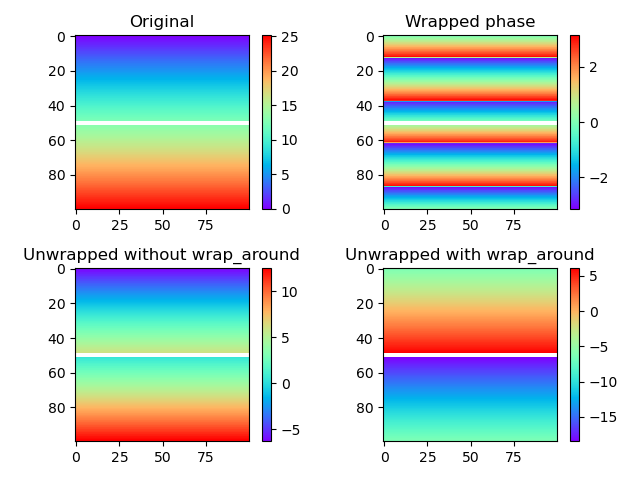
\includegraphics[width=\textwidth]{Images/phase_unwrapping.png}
    \caption{Phase unwrapping with skimage package.}
    \label{fig:phase_unwrap_skimage}
\end{figure}

Firstly, the phase outside a certain threshold (default value 0.05) is set to zero. A different threshold, lower than the isosurface threshold, is used on the amplitude to compute the support so that surface voxels aren't accidentally excluded from the correction.
The phase is then unwrapped, thanks to the skimage method (see figure \ref{fig:phase_unwrap_skimage}). It is then wrapped properly between the maximum and minimum of the phase.

\begin{minted}{python}
    phase, extent_phase = pu.unwrap(
        avg_obj,
        support_threshold=threshold_unwrap_refraction,
        debugging=debug,
        reciprocal_space=False,
        is_orthogonal=is_orthogonal,
    )
    
    extent_phase = phase.max() - phase.min()
    
    phase = (obj - start_angle + range_angle) \% range_angle + start_angle
\end{minted}

Secondly, the phase ramp is removed before phase filtering. To do so, the gradient of the phase is computed in three directions. It returns a set of ndarrays corresponding to the derivatives of the phase with respect to each dimension. Each derivative has the same shape as f.
The points for which the gradient is higher than the threshold ($\approx 1$) are ignored. The mean of the other points is returned as the ramp along that direction.

\begin{minted}{python}
    # Detail below
    amp, phase, rampz, rampy, rampx = pu.remove_ramp(
        amp=abs(avg_obj),
        phase=phase,
        initial_shape=original_size,
        method="gradient",
        amplitude_threshold=isosurface_strain,
        threshold_gradient=threshold_gradient,
    )
    
    # Define the support from the amplitude
    support = np.where(amp > amplitude_threshold * abs(amp).max(), 
                        1, 0)
    
    # Compute gradient
    gradz, grady, gradx = np.gradient(phase, 1)
    
    # Remove points lower than threshold
    threshold_gradient = 1.0
    supportz = np.where(abs(gradz) < threshold_gradient, 1, 0)
    
    # Make sure there  are no points outside the support
    supportz = supportz * support
    
    # Ramp is the mean value
    rampz = gradz[supportz == 1].mean()
    
    # Create mesh grid
    myz, myy, myx = np.meshgrid(
        np.arange(0, nbz, 1),
        np.arange(0, nby, 1),
        np.arange(0, nbx, 1),
        indexing="ij",
    )
    
    # Remove phase gradient
    phase = phase - myz * myrampz - myy * myrampy - myx * myrampx
\end{minted}

Example of gradient computation in python, using the nearest neighbours, see example applied to object phase in figure \ref{fig:phase_grad}.
\begin{minted}{python}
    f = np.array([1, 2, 4, 7, 11, 16], dtype=float)
    np.gradient(f) = array([1. , 1.5, 2.5, 3.5, 4.5, 5. ])
\end{minted}

\begin{figure}
    \centering
    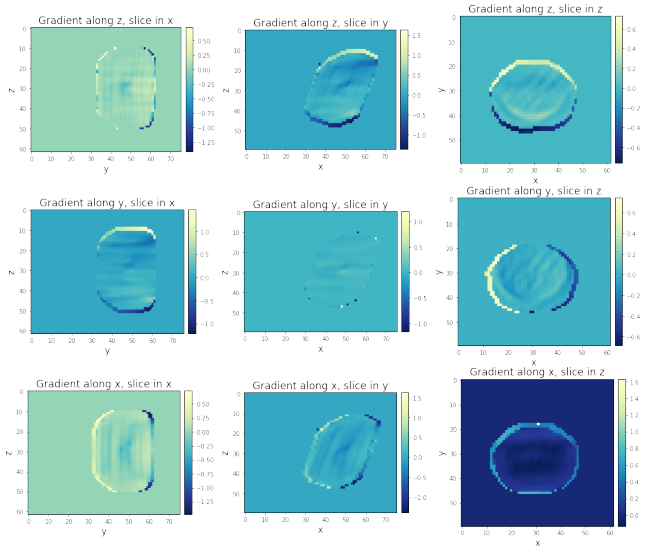
\includegraphics[width=\textwidth]{Images/phase_grad.png}
    \caption{Phase gradients}
    \label{fig:phase_grad}
\end{figure}

Thirdly, the phase offset is removed. Careful here, the threshold used is \verb|isosurface_strain|, the offset is either the value at the COM of the amplitude, or the mean value of the phase.

\begin{minted}{python}
    # Phase offset removal, detail below
    support = np.where(amp > isosurface_strain * amp.max(), 1, 0)
    phase = pu.remove_offset(
        array=phase,
        support=support,
        offset_method=offset_method, # usually mean, or COM
        phase_offset=phase_offset, # usually 0
        offset_origin=offset_origin, # usually not pre-determined
        title="Phase",
        debugging=debug,
    )
    
    # COM
    if offset_method == "com":
        zcom, ycom, xcom = center_of_mass(support)
        array = array - array[zcom, ycom, xcom] + phase_offset
    # mean
    elif offset_method == "mean":
        array = array - array[support == 1].mean() + phase_offset
        
     # wrap again
     phase = (phase - start_angle + range_angle) \% range_angle + start_angle
\end{minted}

Once that the phase is unwrapped, and that the phase ramp and offset are removed, the phase is averaged over a window and apodized to reduce noise in strain plots. The phase is averaged using a kernel of half-width \verb|half_width_avg_phase|. For the apodization, the diffraction pattern is recomputed with \verb|numpy.fft.fftn()|. This function computes the N-dimensional discrete Fourier Transform over any number of axes in an M-dimensional array by means of the Fast Fourier Transform (FFT). The zero-frequency component is shifted to the center of the spectrum using \verb|numpy.fft.fftshift()|.
An apodization window 

\begin{minted}{python}
    # compute support
    support = np.where(amp < isosurface_strain, 1, 0)
    
    # Average phase with nearest neighbours
    phase = pu.mean_filter(
        array=phase, support=support, 
        half_width=half_width_avg_phase, # usually 1
    
    # Apodization
    amp, phase = pu.apodize(
        amp=amp,
        phase=phase,
        initial_shape=original_size,
        window_type=prm.get("apodization_window", "blackman"),
        sigma=prm.get("apodization_sigma", [0.30, 0.30, 0.30]),
        mu=prm.get("apodization_mu", [0.0, 0.0, 0.0]),
        alpha=prm.get("apodization_alpha", [1.0, 1.0, 1.0]),
        is_orthogonal=is_orthogonal,
    )
    
    # Compute electronic density
    avg_obj = amp * np.exp(1j * phase)
\end{minted}
    
The phase is now corrected. The following steps are the centering of the object, as well as the interpolation of the arrays in the orthogonal reference frame where $\vec{q_{com}}$ is aligned onto the reference axis.
\begin{minted}{python}
    # Centering of array
    if centering_method == "max":
        avg_obj = pu.center_max(avg_obj)
        # shift based on max value,
        # required if it spans across the edge of the array before COM
    elif centering_method == "com":
        avg_obj = pu.center_com(avg_obj)
    elif centering_method == "max_com":
        avg_obj = pu.center_max(avg_obj)
        avg_obj = pu.center_com(avg_obj)
        
    # Calculate q of the Bragg peak in the laboratory frame
    q_lab = (
        setup.q_laboratory
    )  # (1/A), in the laboratory frame z downstream, y vertical, x outboard
    qnorm = np.linalg.norm(q_lab)
    q_lab = q_lab / qnorm
    
    # Find Bragg peak
    bragg_peak = bu.find_bragg(
        data=data,
        peak_method="maxcom",
        roi=detector.roi,
        binning=None,
    )
    
    # Compute atomic planar distance
    planar_dist = 2 * np.pi / qnorm  # qnorm should be in angstroms
    planar_dist = planar_dist / 10  # switch to nm
        
    # Find inplane and outofplane angles from setup
    # and Bragg peak
    setup.correct_detector_angles(bragg_peak_position=bragg_peak)
    prm["outofplane_angle"] = setup.outofplane_angle
    prm["inplane_angle"] = setup.inplane_angle
        
    # Orthogonalise object
    obj_ortho, voxel_size, transfer_matrix = setup.ortho_directspace(
        arrays=avg_obj,
        q_com=np.array([q_lab[2], q_lab[1], q_lab[0]]),
        initial_shape=original_size,
        voxel_size=fix_voxel,
        reference_axis=axis_to_array_xyz[ref_axis_q],
        fill_value=0,
        debugging=True,
        title="amplitude",
    )
\end{minted}

The orthogonalised object is re-centered on its center of mass, the phase unwrapping, the phase ramp removal and the phase offset removal are repeated. To resume, \verb|threshold_unwrap_refraction| is only used for the phase unwrapping, whereas  \verb|isosurface_strain| is used for both the phase ramp removal and the phase offset removal.
In order to facilitate the analysis of data-sets collected on the same object, the values of these two parameters should be the same as much as possible. In any case, they should be kept in mind when analysing the data.
Do not forget the -1 sign in the phase if the phasing algorithm is python or matlab-based.
Finally, the strain is computed from the phase.

\begin{minted}{python}
    # Add offsets if defects
    if method == "defect":
        offsets = 2 * np.pi / 10 * np.linspace(-10, 10, num=11)
    else:
        offsets = (0,)
        
    for offset in offsets:
        # offset the phase
        if method == "defect":
            temp_phase = np.copy(phase)
            temp_phase = temp_phase + offset
            # wrap again the offseted phase
            temp_phase = util.wrap(
                obj=temp_phase,
                start_angle=-extent_phase / 2,
                range_angle=extent_phase
            )
        else:  # no need to copy the phase, offset = 0
            temp_phase = phase

        # calculate the strain for this offset,
        # disp = planar_distance / (2 * np.pi) * temp_phase,
        if reference_axis == "x":
            _, _, temp_strain = np.gradient(
                planar_distance / (2 * np.pi) * temp_phase,
                voxel_size[2],
            )  # q is along x after rotating the crystal
        elif reference_axis == "y":
            _, temp_strain, _ = np.gradient(
                planar_distance / (2 * np.pi) * temp_phase,
                voxel_size[1],
            )  # q is along y after rotating the crystal
        else:  # "z"
            temp_strain, _, _ = np.gradient(
                planar_distance / (2 * np.pi) * temp_phase,
                voxel_size[0],
            )  # q is along z after rotating the crystal

        # update the strain values
        strain = np.where(abs(strain) < abs(temp_strain), strain, temp_strain)
\end{minted}


\subsubsection{\textit{Gwaihir}}